\documentclass[tikz,border=3.14mm]{standalone}
\usepackage{amssymb,mathrsfs}

\begin{document}
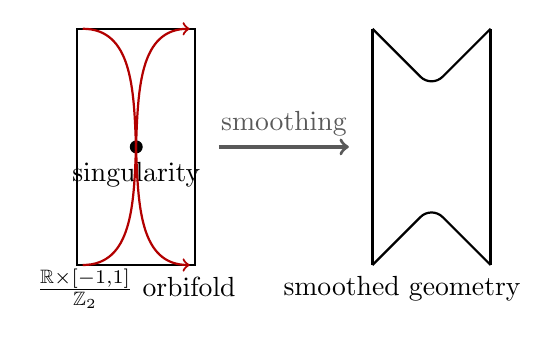
\begin{tikzpicture}[scale=1.5]
  % Orbifold (left)
  \draw[thick] (0, -1) rectangle (1, 1);
  \filldraw[black] (0.5, 0) circle (0.05) node[below=2pt] {singularity};
  
  % Identifications for orbifold
  \draw[->, thick, red!70!black, shorten >=2pt, shorten <=2pt] (0, 1) to[out=0, in=180] (1, -1);
  \draw[->, thick, red!70!black, shorten >=2pt, shorten <=2pt] (0, -1) to[out=0, in=180] (1, 1);
  
  % Smoothed geometry (right)
  \begin{scope}[xshift=2.5cm]
    \draw[thick, rounded corners=0.2cm] (0, -1) -- (0.2, -0.8) -- (0.5, -0.5) -- (0.8, -0.8) -- (1, -1);
    \draw[thick, rounded corners=0.2cm] (0, 1) -- (0.2, 0.8) -- (0.5, 0.5) -- (0.8, 0.8) -- (1, 1);
    \draw[thick] (0, -1) -- (0, 1);
    \draw[thick] (1, -1) -- (1, 1);
  \end{scope}
  
  % Arrow between figures
  \draw[->, very thick, gray!70!black] (1.2, 0) -- (2.3, 0) node[midway, above] {smoothing};
  
  % Labels
  \node at (0.5, -1.2) {$\frac{\mathbb{R} \times [-1,1]}{\mathbb{Z}_2}$ orbifold};
  \node at (2.75, -1.2) {smoothed geometry};
\end{tikzpicture}
\end{document}